%!TEX root = ../main_wo_rep.tex
%
% 電子の比電荷の測定
%


\section{電子の比電荷の測定}

\subsection{比電荷とは}

電子はマイナスの電荷を持ち、非常に質量の小さい素粒子です。電子の電荷の大き 
さを$e$、電子の質量を$m_e$とするとき、電荷と質量の比:$e/m_e$を測定することを考え 
てみましょう。この、$e/m_e$の値のことを{\bf 比電荷}と言います。比電荷の測定はJ.J.~ト 
ムソンによって行なわれ、トムソンは1906年にノーベル物理学賞を受賞しました。

一方、電子の電荷$e$(電気素量)の値はミリカンによる油滴実験によって初めて測定されました。
ミリカンもこれらの業績によって、1923年にノーベル物理学賞を受賞しています。
電気素量は過去多くの
実験により、精密に測定されてきましたが、現在では
国際単位系(SI)により次の値として厳密に定められています。
\begin{center}
\fbox{電気素量: $e=\text{1.602 176 634}\times10^{-19}$ [C (クーロン)]}
\end{center}

比電荷の測定を行い、定義された電気素量の値を用いると、電子の質量を決定することができます。
ここでは比電荷の測定を実際に行ない、電気素量$e$の値を用いて電子の質量を導出 
しましょう。

\subsection{測定原理}

まず、フィラメント(ヒーター)を加熱し熱電子を放出します。
次に、この電子を速度$v$まで加速させます。加速する為には、電子に電圧$V$をかけ
ます。電子の運動エネルギーと加速電圧$V$の間の関係式は、
\[
\frac{1}{2}m_ev^2 = e V
\]
で与えられるので、この式から加速電圧$V$で加速された電子の速度は、
\begin{equation}
v^2=\frac{2eV}{m_e}
\label{v square}
\end{equation}
となります。このように熱電子を電圧によって加速して打ち出す一連の装置のことを電子銃といいます。

\newpage

\begin{wrapfigure}[8]{r}{5cm}
\vspace*{-0.5cm}
\hspace*{0.5cm}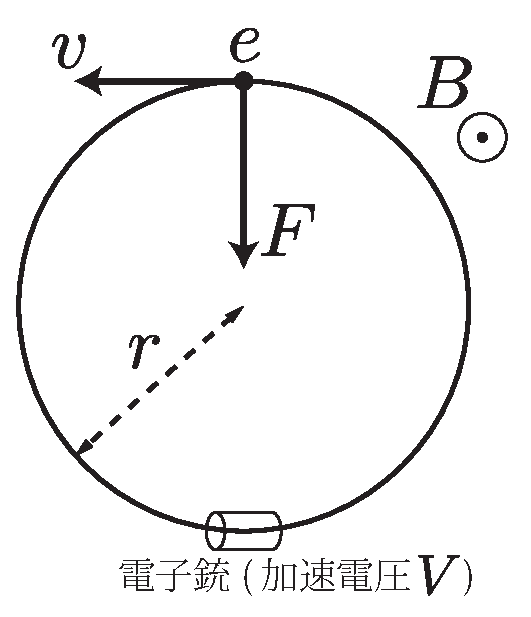
\includegraphics[scale=0.5]{11_CTMratio/CTMratio.eps}\\
$\odot$は向こう側から手前に向かっている矢印を表します。
\end{wrapfigure}

さらに、この速度$v$で動いている電子に磁場をかけると、
右図のように、電子に対してローレンツ力(フレミングの左
手の法則で表わされる力)が働きます。このローレンツ力が
電子に働く遠心力とつりあい、電子の軌道が半径$r$の円を描
くようになります。この実験では、ヘルムホルツコイルと呼
ばれるコイルに電流を流すことによって磁場を作り出します。


磁束密度の大きさを$B$とすると、ローレンツ力は、
\[
F=evB
\]
となるため、ローレンツ力と遠心力のつりあいの式は次のようになります。
\begin{equation}
evB=\frac{m_e v^2}{r}
\label{evB}
\end{equation}

(\ref{v square})式、(\ref{evB})式から電子の速度$v$を消去すると、
\begin{equation}
\boxed{
\frac{e}{m_e}=\frac{2V}{B^2r^2}
}
\end{equation}
となります。この式から、電子の加速電圧$V$、磁束密度の大きさ$B$、電子の軌道半径$r$ 
を測定すれば、電子の比電荷が求められることが分かります。

磁束密度の大きさ$B$とヘルムホルツコイルに流れる電流$I$の関係は、コイルの半径や巻数によ
って決まっており、ここで用いる装置では、
\begin{equation}
\boxed{
B=7.80\times 10^{-4}\times I
}
\end{equation}
の関係があります。(ただし、$B$の単位は[Wb/m${}^2$]。) 



\bigskip

\begin{itembox}[l]{\bf コラム:電気素量の決定}
電子の電荷を最初に測定したのは、アメリカ人のミリカンである。静電気を持った(電
子の付着した)油滴が電場の中で落下する様子を観測することで測定に成功した。重力
によって自然に落下している油滴に重力と逆向きに電場をかけると、クーロン力によっ
て落下速度が減速される。その速度を測定することでクーロン力の大きさがわかり、あ
らかじめ知っている電場の大きさを使って油滴についている静電気の量が求められる。
この実験を様々な油滴について行うと、油滴についている電気量は油滴ごとに異なるが、
いずれの場合も、ある量の整数倍となる。この``ある量''の存在が``電気の粒''のよう
なものがあることを示唆し、この``電気の粒''が電子であり、``ある量''は電子1個が
持つ電気量である。ちなみに、知られている粒子の電荷はすべて電子の電荷の整数倍に
なっているので、電子の電荷を電気素量とよぶ。
\end{itembox}

\newpage

\jikken

\begin{itemsquarebox}[c]{\bf 実験用具}
電子の比電荷測定器、真空管用電源装置、直流安定化電源装置、直流電流計
($\sim$5[A])、直流電圧計($\sim$ 1000[V])、接続用ケーブル、棒磁石
\end{itemsquarebox}

\bigskip

\subjikken{電子の比電荷の測定}

\begin{enumerate}

\item まず、装置の説明書を読み、実験装置を接続しましょう。(\underline{配線が終了するまで、} \\
\underline{絶対に電源を入れないこと!} 接続が完了したら、電源を入れる前に配線を確認 
しますので、必ず声をかけてください。)

\item 真空管用電源装置の電源を入れ、B電圧つまみを回して、電圧を150$\sim$300[V]に 
します。(電子のビームが見えるので、必要があれば焦点を調整します。)

\item 電子ビームの棒磁石を近づけローレンツ力が働いていることを確認してみましょう。

\item 直流安定化電源装置の電源を入れ、「Voltage」つまみを回して6[V]$\sim$9[V]の間に 
します。比電荷測定装置のヘルムホルツコイルの電流調整つまみをゆっくり回し、 
電流を流していくと磁場が発生し、ビームが円を描くようになります。


\item 測定は次の手順で行います。

\begin{enumerate}

\item 加速電圧をまず150 [V]に固定し、ヘルムホルツコイルに流れる電流を変 
化させながら、電子の軌道が円になった所でのコイルの電流と円の半径を 
測定します。(実際には円の直径を求め、それを2で割って半径を求めれ 
ば良い。)

\item コイルに流す電流を一定の間隔で増加させながら、電流と電子の軌道の半 
径を記録していきます。(1$\sim$1.5[A]程度まで)

\item 加速電圧を50[V]きざみで大きくして、1)と2)の操作を繰り返します。 
(300[V]まで)

\end{enumerate}

\item 得られたデータを整理し、比電荷の値をそれぞれ求め、平均値を求めましょう。 
また、電子の電荷を$e=1.6022\times 10^{-19}$[C]として、電子の質量を求めましょう。


\end{enumerate}
